% 15 de mayo de 2018
\chapter{Presentación y discusión de la información}\label{ch:informacion}

El proceso de entrevistas fue realizado entre los meses de abril y septiembre
del año 2017.
Estas entrevistas fueron transcritas para su análisis en el texto.
Los elementos expresados por los participantes en las entrevistas fueron
codificados y organizados en las categorías y subcategorías que se pueden
observar en la figura~\ref{fig:categorias}.
Las entrevistas fueron codificadas empleando el programa ATLAS.TI en su versión
7.5.7 proceso que facilitó la categorización de la información recolectada a lo
largo de las entrevistas.

\begin{figure}
    \centering
    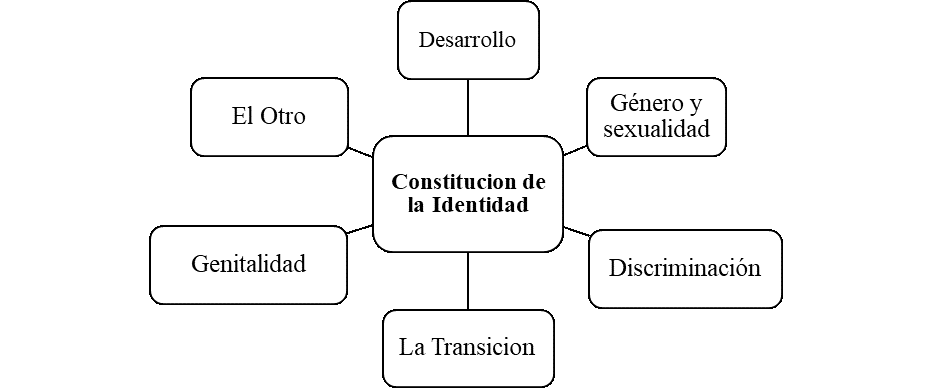
\includegraphics[width=0.75\textwidth]{categorias}
    \caption{Diagrama de categorías}\label{fig:categorias}
\end{figure}

A continuación realizaremos una descripción de cada una de ellas junto con los
verbatim que les dan origen.
Adicionalmente presentamos el razonamiento e interpretación que damos a cada
categoría y sus implicaciones caso a caso para el cumplimiento de los objetivos
de investigación.
El orden de presentación de las mismas fue elegido
según la frecuencia de manifestación en las entrevistas realizadas.

En la sección~\ref{sec:discusion}, realizamos una discusión y análisis punto a
punto de cada una de las categorías.

\section{Presentación de la información}

Como se puede ver resumido en la figura~\ref{fig:categorias}, hemos elaborado
seis (6) categorías. Dentro de estas categorías ‘La transición’ es uno de los
componentes identificados como constitutivo del proceso de construcción de la
identidad de las personas trans. Procederemos a explorar el contenido de cada
una de las categorías identificadas.

\subsection{Desarrollo}
Esta categoría se encuentra compuesta por elementos que abarcan desde etapas
tempranas de la niñez y del desarrollo.
Elementos como la relación del individuo con su escolaridad y compañeros de
clases.
También elementos de la constitución de los géneros que se hacen presentes
dentro de la pubertad y los conflictos que estos puedan causar a los
participantes
También incluye el papel que juega la familia dentro de la constitución de la
identidad así como la forma de aproximarse a los problemas.
Todos estos son elementos que pueden marcar la construcción de identidad de una
persona.

\begin{figure}
    \centering
    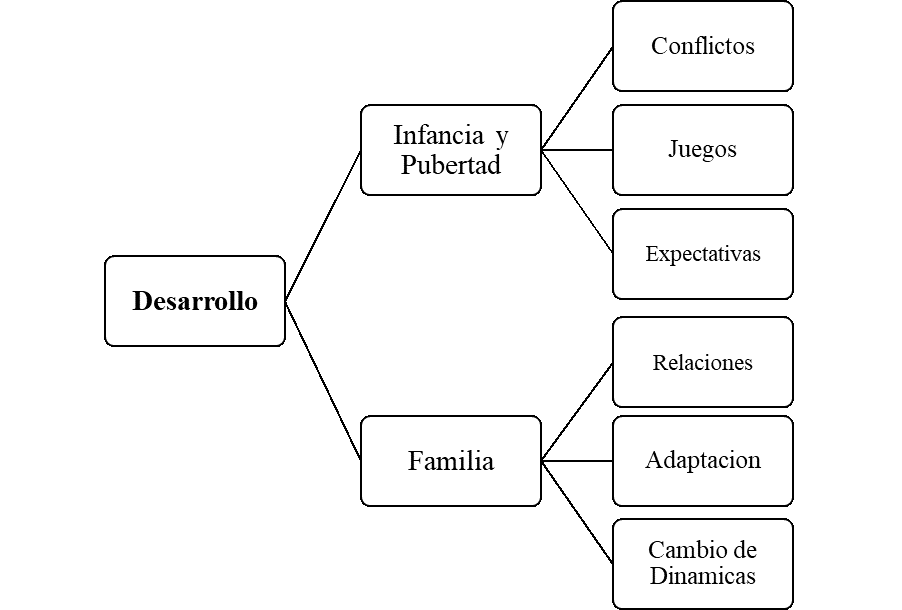
\includegraphics[width=0.75\textwidth]{desarrollo}
    \caption{Diagrama ‘desarrollo y familia’}\label{fig:desarrollo}
\end{figure}

En esta categoría confluyen elementos de conflicto así como las experiencias que
permitieron el manejo de los mismos en los participantes y que
consecuentemente se transformaron en estrategias de afrontamiento. Se debe tomar
en cuenta que en esta categoría se presentan los distintos tipos de relación
establecidas tanto en niveles académicos como familiares entre la infancia y
pubertad de los participantes.

Existen dos subcategorías dentro de este factor. Una de ‘infancia y pubertad’,
que reporta sobre las experiencias de desarrollo y formativas en la juventud, y
otra de ‘familia’. Esta habla acerca de la influencia de los lazos y ambiente
familiar durante el desarrollo.

\subsubsection{Infancia y pubertad}
Dentro de esta subcategoría se pueden
encontrar elementos que parecen ser transversales a lo largo de la vida del
individuo. Al ser tanto la infancia como la pubertad etapas tempranas de
desarrollo y constitución se pudo identificar elementos que parecen sentar las
bases para la forma otros elementos que le permiten al individuo constituirse
como persona. Entre estos elementos cabe resaltar la presencia de conflictos
como lo expresa el Sujeto 1 (verbatim):

\begin{verbatim}
…bueno me identificaba como niño pero me gustaba todo las cosas
de niña. De hecho siempre pedía al niño Jesús cosas de hembra, por ejemplo,
barbie, oso etcétera,  por su puesto jamás me traía lo que pedía y era muy
triste para mí, una era inocente y el niño Jesús me dejaba una carta explicando
que eso eran cosas de niña y me traía patineta bicicleta carrito y a mí no me
gustaba…
\end{verbatim}

Este elemento puede estar ligado al rechazo que pueden vivir, según lo expresado
por Sujeto 1 (verbatim):

\begin{verbatim}
…en la escuela era algo terrible por el bullying, pero yo
siempre imponía carácter y jamás me deje amedrentar por nada ni nadie.  De hecho
me agarre a golpes y me expulsaron por 10 días…
\end{verbatim}

O a tener su raíz en conflictos por la constitución de su identidad como lo
expresan con los siguientes verbatims.

Sujeto 1:
\begin{verbatim}
…yo lloraba porque no me entendía y me sentía mal.
\end{verbatim}

Sujeto 2:

\begin{verbatim}
  …me criticaban mucho como me vestía, pero es lo que me gusta.
\end{verbatim}

Y sujeto 3:

\begin{verbatim}
…siempre era el raro del grupo…
\end{verbatim}

La aparición de estos conflictos entra en contacto con las aproximaciones a los
roles de género que suceden por primera vez en la infancia por medio de los
juegos y que perduran a lo largo de la vida de un individuo, como se evidencia
en el relato de Sujeto 1:

\begin{verbatim}
…a mí me decían que tenía que jugar con carritos y no con
muñecas porque eso es de niñas y yo no era una…
\end{verbatim}

Y del Sujeto 3:

\begin{verbatim}
…me gustaba tener el cabello corto y no me arreglaba pero mis
padres me decían que tenía que arreglarme para poder verme linda…
\end{verbatim}

 Un elemento que se ve relacionado con la presencia del conflicto de identidad
 es que la aprehensión del mismo lleva al individuo a buscar o considerar el
 daño que puede causar el no lidiar con esta situación y es por eso que hay
 comentarios como el emitido por el Sujeto 3 quien expresa:

 \begin{verbatim}
Descubrí que tenía que hablar de esto con alguien o me iba a volver loco.
 \end{verbatim}

 Este verbatim, trae a la luz el malestar que nace en el individuo por este
 conflicto de identidad, posiblemente el hecho de estar en una situación de la
 cual se tiene poca o ninguna información al alcance del individuo hace que el
 malestar por el conflicto sea mayor y pueda tener consecuencias mas peligrosas
 para la identidad de la vida del individuo.

\subsubsection{Familia}

Otro de los componentes de la categoría ‘Desarrollo’ es la subcategoría
denominada \emph{Familia}, pues según  lo expresado por los individuos como
Sujeto 3:

\begin{verbatim}
…en mi casa siempre era un conflicto hablar sobre cómo me sentía.
\end{verbatim}

Sujeto 2:

\begin{verbatim}
Mi mamá me decía, ‘hija arréglate un poco’ ó ‘te verías muy linda
con vestido’ y yo le decía que no me gustaba eso y venia el regaño.
\end{verbatim}

Esta subcategoría influye en la constitución del individuo y modela su
desarrollo, en aspectos como la forma de establecer relaciones,
tomando lo expresado por Sujeto 2:

\begin{verbatim}
…la relación con mis padres es distinta, a mi madre le costó más
aceptarme, a mi padre después de explicarle lo entendió con más facilidad,
incluso suelo pasar por su trabajo, es moto taxista.
\end{verbatim}

Un elemento que resaltan los participantes es el cambio de dinámicas dentro de
la familia que se da producto de asumirse como persona trans. Como se observa en
el relato de Sujeto 1:

\begin{verbatim}
…mi madre al principio le costó mucho aceptarlo y mi papa le
dijo a mis hermano que porque no me quedaba como yo. Era que él me aceptaba gay
mas no vestido de mujer y jamás me permitió aclararle los conceptos que tenía
errado y hasta hoy no me trata ni mi padre ni mi hermano menor…
\end{verbatim}

Estos verbatims asoman que dentro de las familias de los individuos transgéneros
existe una innegable presencia de conflicto generado por la nueva identidad
asumida por el mismo. El cómo esta identidad interactúa con las prenociones de
la familia suma a la conflictividad durante el desarrollo. Es posible que esta
situación este relacionada con el propio conflicto interno que pueden vivir
personas transgénero como consecuencia de la falta de acceso a información que
permita aclarar sus dudas.

Esto podría ser un indicador de las percepciones hegemónicas sobre la sexualidad
y como estas moldean las diversas interacciones entre los individuos. Se
observa en el verbatim del Sujeto 1 que por parte de su padre existe aún una
confusion entre lo que es la orientación (los gustos del individuo) y su
identidad (como el individuo se observa a sí mismo) sexual.

\subsection{Género y sexualidad}

La siguiente categoría que permite la constitución de identidad en los
participantes es la de \emph{género y sexualidad}. En esta categoría se
presentan elementos como la constitución de la identidad que tienen su raíz en
etapas tempranas de la vida, con base a lo expresado por los participantes se
generaron las siguientes subategorias: Identidad de género, Hegemonía de género
y Orientación Sexual.

En la figura~\ref{fig:genero} se puede observar los elementos constitutivos de
la categoría.

\begin{figure}
    \centering
    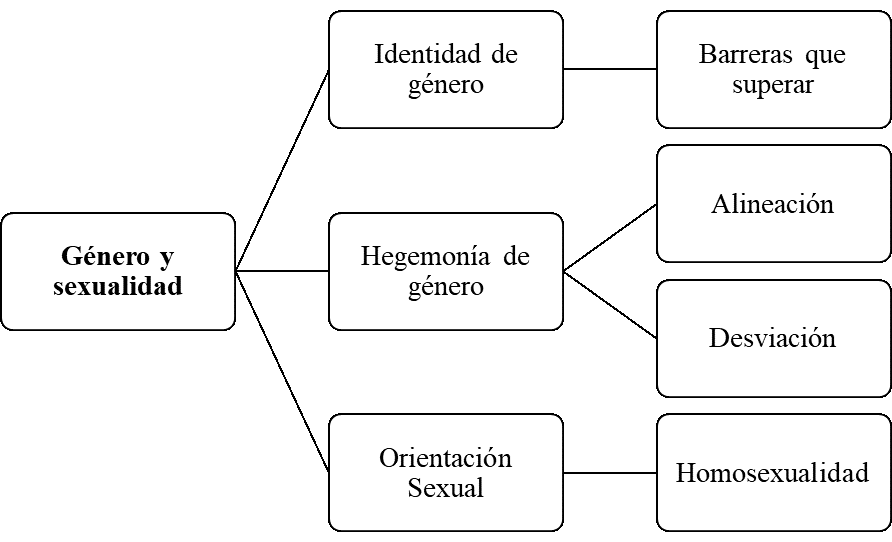
\includegraphics[width=0.75\textwidth]{genero}
    \caption{Diagrama de ‘género y sexualidad’}\label{fig:genero}
\end{figure}

\subsubsection{Identidad de género}

Esta subcategoría se mostró como la más importante dentro de lo expresado por
los participantes principalmente porque ha sido el componente central con
el que se enfrentaron en la constitución de su identidad. Esto se puede ver
reflejado en lo expresado por Sujeto 2:

\begin{verbatim}
…el momento más feliz de mi infancia es cuando me pude vestir
de Ángel Gabriel en un nacimiento viviente que hicieron en mi escuela. Mi mamá
no quería pero yo me sentía en las nubes porque por un momentito pude verme como
quería.
\end{verbatim}

Este conflicto de identidad también se hace visible dentro del relato de Sujeto
3 cuando expresa:

\begin{verbatim}
…no es que solo me gustaba vestirme como hombre, es que pensaba
como uno también.
\end{verbatim}

Así como dentro del relato de Sujeto 1 cuando comenta:

\begin{verbatim}
Cuando era pequeña no me molestaba, pero cuando empecé a
desarrollarme le rezaba a Dios para que por favor me salieran senos.
\end{verbatim}

Estos verbatims permiten identificar algunos aspectos relacionados con el
conflicto de identidad de los individuos. Elementos como el verbatim expresado
por el Sujeto 2 que considera un recuerdo muy feliz el poder mostrar una
expresión de género acorde a la identidad que, ya para esa etapa de su
desarrollo, sentía era la de él. Además esto se puede reforzar con el verbatim
del Sujeto 1 cuando expresa que le causaba preocupación y ansiedad el hecho que
sus senos no se desarrollaran junto con el resto de su cuerpo.

Además se presenta la dicotomía entre lo que las personas sienten que son, las
expectativas de como esperan verse y la imposición de la identidad que se
les asigno por haber nacido con un sexo especifico.

\subsubsection{Hegemonía de género}

\subsubsection{Orientación sexual}

\subsection{Discriminación}
% TODO Emerson arreglará
\begin{figure}
    \centering
    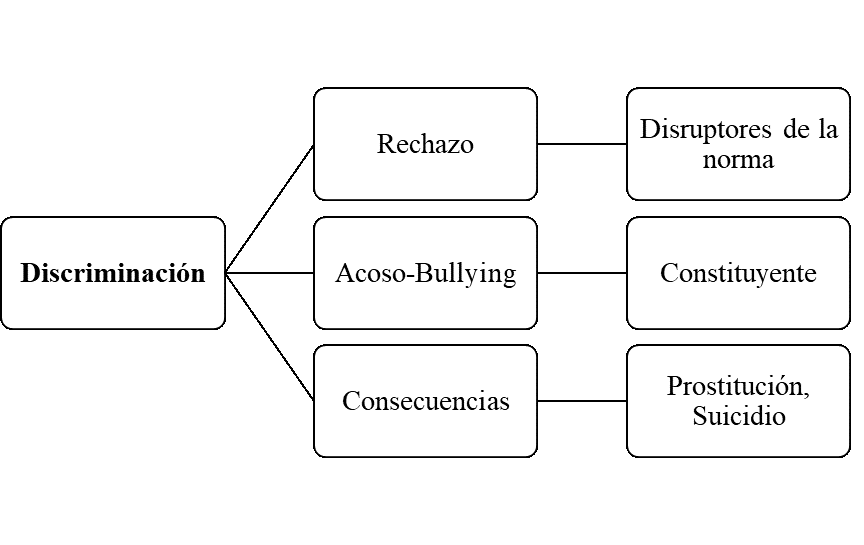
\includegraphics[width=0.75\textwidth]{discriminacion}
    \caption{Diagrama de categoría ‘discriminación’}\label{fig:discriminacion}
\end{figure}


\subsubsection{Rechazo}

\subsubsection{Acoso / Bullying}

\subsubsection{Consecuencias}

\subsection{La Transición}
% TODO limpiar redacción y extender
Esta categoría comprende elementos relacionados con
el tránsito entre un género o sexo a otro, los cuales abarcan desde la
elaboración desde la subjetividad que los sujetos hacen sobre el transitar hasta
elementos como lo son la apariencia física o el conocimiento de los procesos que
permiten la transición.

\begin{figure}
    \centering
    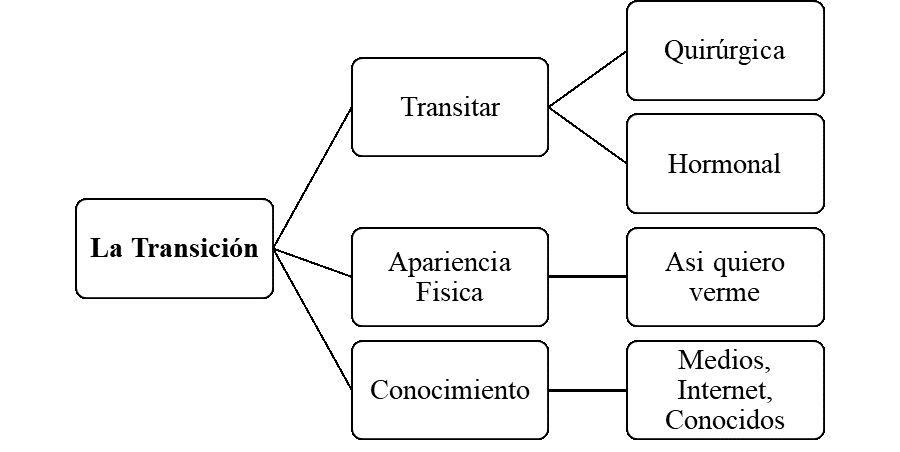
\includegraphics[width=0.75\textwidth]{transicion}
    \caption{Diagrama de ‘la transición’}\label{fig:transicion}
\end{figure}

\subsubsection{Transitar}

Según lo expresado por los participantes, el transitar es mas allá de un hecho
una herramienta. La transición es un medio que les permite llega a ser quien
ellos sienten que son. El poder transitar puede abarcar aspectos quirúrgicos y/u
hormonales, y como lo expresa Sujeto 2:

\begin{verbatim}
…las hormonas ayudan pero la operación libera…
\end{verbatim}

Sujeto 3 coincide al comentar:

\begin{verbatim}
…las hormonas ayudan, cuando dejé de tomarlas perdí todo, era una niña…
\end{verbatim}

Estos evidencia que existe una valoración de la alteración quirúrgica como más
importante que la transición hormonal. Además se considera la transición
quirúrgica como un objetivo final o como una acción liberadora.

Sin embargo, lo dicho por el sujeto 3 hace referencia a como el componente
hormonal tiene una importancia por su cualidad inmediata. Debido a que permite
una visibilización a corto plazo de la identidad mas explicita que una
operación. Los efectos de la transición hormonal son visibles mientras que la
cirugía genital no lo es.

Por otro lado se tiene que tomar en cuenta lo expresado por Sujeto 1:

\begin{verbatim}
…por cuanto mi apariencia física y genética me han ayudado en la transición lo
cual ha sido muy fácil, de hecho no he tomado hormona nunca…
\end{verbatim}

Esto permite indicar que la importancia no está colocada en la toma de hormonas
en sí mismo. Sino que la importancia está en los cambios de aspecto físico y de
visibilidad que se producen como resultado de la influencia hormonal. En este
caso la sujeto 1 indica no necesitar de la toma hormonal pues su aspecto ya es
femenino en sí, lo que es su objetivo último.

\subsubsection{Apariencia física}

Dentro de esta subcategoría se encuentra todos los elementos relacionados con la
expresión de la relación sexo-género, tomando en cuenta que dentro de esta
relación hay particularidades que tienen un mayor peso o que suelen tomarse más
en cuenta para su expresión como lo plantea por ejemplo Sujeto 3:

\begin{verbatim}
  …perdí el torso perdí básicamente eso, la libido cambio…
\end{verbatim}

Esto implica que es poder verse y expresarse en concordancia con los
rasgos del sexo o género al que se transita es fundamental. Además de esto se
puede tomar en cuenta lo expresado por Sujeto 2:

\begin{verbatim}
…le tengo terror a la regla porque soy hombre y a los hombres no les debe venir
eso.
\end{verbatim}

Elemento que puede servir para ampliar la concepción de concordancia de
sexo/género, pues estar alineado no solo puede significar tener características
propias de un sexo o género, sino que también puede significar no tener o evitar
las asociadas con otro.

\subsubsection{Conocimiento}

La subcategoría de conocimiento hace referencia tanto a como los participantes
reafirmaron o conocieron su condición así la manera con la cual entraron en
contacto con el proceso que les permitiese su transición. En esta subcategoría
parece resaltar el papel de los medios para visibilizar la condición trans,
Sujeto 2 expresa que:

\begin{verbatim}
…yo no conocía de lo trans ni nada, pensaba que era homosexual y ya, pero
luego un día viendo televisión con mi novia de ese momento pasaron el primer
capítulo del programa ‘Taboo’, por NatGeo y ahí presentaron a una persona trans
y mi novia me dijo, mira ella dice que se sentía como tú dices que te sientes
y pues eso me dejó pensando.
\end{verbatim}

Por otro lado se puede tomar como referente la experiencia de Sujeto 1 que
expresa:

\begin{verbatim}
Me di cuenta y logre comprender que era ser trans a los 40 años de edad, porque
desconocía que era ser trans, de hecho en mi ignorancia tampoco sentía que me
identificaba como gay porque me sentía mujer pensaba como mujer y eso no lo
entendía, todo eso lo viví en silencio por 40 años jamás dije nada por el
rechazo que pudiera sentir hasta que me hablaron de personas trans y fue allí
cuando comencé a entender que yo era una mujer transexual.
\end{verbatim}

El Sujeto 1 añade:

\begin{verbatim}
Lo descubrí a los 40 años gracias a mi psicólogo que me realizo una terapia y
allí fui abriéndome y diciendo lo que sentía y fue cuando supe que era una mujer
trans.
\end{verbatim}

Esto potencia el rol del psicólogo como voz autorizada y mediador en el proceso
de transición, calmando el malestar del individuo.

\subsection{Genitalidad}

Esta categoría se centra en el aspecto biológico de la identidad del individuo
pero no abarca componentes hormonales o cromosómicos como tales sino que se
centra únicamente en el aspecto físico genital desde lo visual y lo sensitivo
así como lo que representa para los participantes este aspecto de su cuerpo.

\begin{figure}
    \centering
    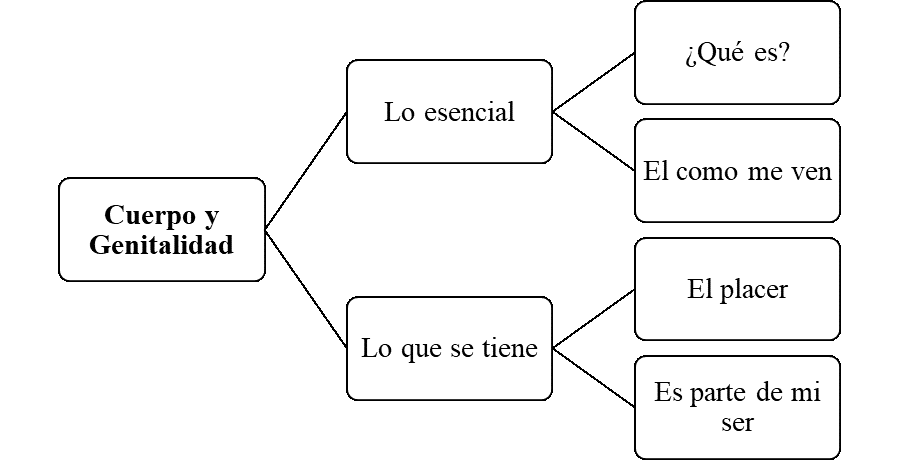
\includegraphics[width=0.75\textwidth]{genitalidad}
    \caption{Diagrama de ‘genitalidad’}\label{fig:genitalidad}
\end{figure}

\subsubsection{Lo esencial}

Esta subcategorías intenta abarcar aquello que los participantes consideraron de
mayor importancia sobre su relación con la genitalidad, es interesante observar
que el componente genital no tiene una primacía en la construcción de su
identidad. Si se toma en cuenta lo expresado por Sujeto 1:

\begin{verbatim}
  Solo me decidí operar el pecho y ponerme mamas.
\end{verbatim}

También por el Sujeto 3:

\begin{verbatim}
¿Para qué un trans se opera el pecho? para poder quitarse la camisa.
\end{verbatim}

Y en especial lo expresado por Sujeto 2:
\begin{verbatim}
Quiero poder operarme para poder quitarme la camisa y hacer cosas normales.
\end{verbatim}

Parece resaltar la importancia de lo que se considera caracteres sexuales
secundarios sobre los primarios, es decir parece ser mas resaltante lo que ve el
otro en público que lo que se ve en privado, comentarios como el de Sujeto 2:

\begin{verbatim}
…a mí me encanta ir al gimnasio y tener la espalda ancha, me
siento como un monstruo.
\end{verbatim}

Refuerzan esto, ya que demuestra que lo esencial es mostrarse para todos no para
alguien en especial.

\subsubsection{Lo que se tiene}

\subsection{El Otro}

\begin{figure}
    \centering
    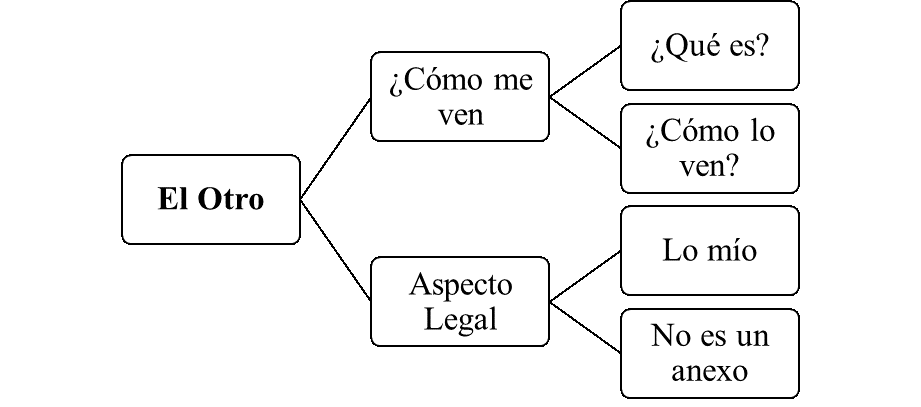
\includegraphics[width=0.75\textwidth]{otro}
    \caption{Diagrama de categoría ‘el otro’}\label{fig:otro}
\end{figure}


\subsubsection{Cómo me ven}

\subsubsection{Aspecto legal}

\section{Discusión}\label{sec:discusion}

\subsection{Desarrollo}

\subsubsection{Infancia y pubertad}

\subsubsection{Familia}

\subsection{Género y sexualidad}

\subsubsection{Hegemonía de género}

\subsubsection{Orientación sexual}

\subsection{Discriminación}

\subsubsection{Rechazo}

\subsubsection{Acoso / Bullying}

\subsubsection{Consecuencias}

\subsection{La transición}

\subsubsection{Transitar}

\subsubsection{Apariencia física}

\subsubsection{Conocimiento}

\subsection{Genitalidad}

\subsubsection{Lo esencial}

\subsubsection{Lo que se tiene}

\subsection{El Otro}

\subsubsection{Cómo me ven}

\subsubsection{Aspecto legal}
